\documentclass[12pt]{beamer}
\usetheme{CambridgeUS}
\usepackage[utf8]{inputenc}
\usepackage[spanish]{babel}
\usepackage{amsmath}
\usepackage{amsfonts}
\usepackage{amssymb}
\usepackage{graphicx}
\usepackage{ragged2e}
\setbeamertemplate{navigation symbols}{} 
\author[Kevin García - Alejandro Vargas]{Kevin García 1533173 \newline Alejandro Vargas 1525953}
\title[Tarea 5: Regresión Robusta]{Tarea 5:Diagnósticos en el Análisis de Regresión, Regresión a Través del Origen y Regresión Robusta}



%\setbeamercovered{transparent} 
%\setbeamertemplate{navigation symbols}{} 
%\logo{} 
%\institute{} 
%\date{} 
%\subject{} 
\begin{document}
\justify
\begin{frame}
\titlepage
\end{frame}

%\begin{frame}
%\tableofcontents
%\end{frame}
\begin{frame}
\frametitle{Introducción}
~\\En esta presentación se tratara de encontrar un modelo lineal adecuado, para predecir la cantidad de $PM_{2.5}$ a partir de la cantidad de $PM_{10}$, para ello se ajustara un modelo simple por MCO y se llevaran a cabo pruebas de diagnostico para detectar e identificar puntos con altos residuales, atípicos, influyentes o de alto leverage, y se tratará de mejorar el modelo llevando a cabo un modelo ajustado que pase por el origen, al cuál se le aplicaran nuevamente las pruebas de diagnostico y se le evaluaran el cumplimiento de los supuestos.Finalmente, se aplicara regresión robusta y se compararan todos los modelos, eligiendo el mejor o el más adecuado.
\end{frame}

\begin{frame}
\frametitle{Definiciones}
~\\El material particulado respirable presente en la atmósfera de nuestras ciudades en forma sólida o líquida (polvo, cenizas, hollín, partículas metálicas, cemento y polen, entre otras) se puede dividir, según su tamaño, en dos grupos principales. A las de diámetro aerodinámico igual o inferior a los 10 $\mu m$ o 10 micrómetros (1 $\mu m$ corresponde a la milésima parte de un milímetro) se las denomina $PM_{10}$ (partículas respirables) y a la fracción respirable más pequeña, $PM_{2.5}$ (partículas finas). Estas últimas están constituidas por aquellas partículas de diámetro aerodinámico inferior o igual a los 2.5 micrómetros, es decir, son 100 veces más delgadas que un cabello humano, además son más peligrosas, ya que, al ser inhaladas, pueden alcanzar las zonas periféricas de los bronquiolos y alterar el intercambio pulmonar de gases.
\end{frame}

\begin{frame}
\frametitle{Modelo Ajustado}
~\\~\\Para ajustar un modelo lineal para estas partículas, decidimos que la variable independiente o regresora fuera el $PM_{10}$ y la variable dependiente fuera el $PM_{2.5}$, se hizo esta selección, ya que las partículas con un diámetro menor o igual a 10 micrómetros son más fáciles de medir que las de diámetro menor o igual a 2.5 micrómetros, y la idea es que se ahorren costos y esfuerzo humano adicional, midiendo solo las partículas $PM_{10}$ (que son un poco más grandes) y a partir de ellas logren obtener una buena estimación para las partículas $PM_{2.5}$.
\end{frame}

\begin{frame}
\frametitle{Modelo Ajustado}
~\\Teniendo en cuenta lo anterior, el modelo planteado es:
$$PM_{2.5}=\beta_{0}+\beta_{1}PM_{10}$$
~\\El modelo ajustado, usando MCO es:
$$\hat{PM_{2.5}}=-4.29990+0.45776PM_{10}$$
\end{frame}

\begin{frame}
\frametitle{Bondad del modelo}
~\\Para este modelo ajustado, tenemos los siguientes resultados que nos ayudaran a juzgar que tan bueno es:
\begin{center}
~\\\begin{tabular}{|c|c|c|c|c|}
\hline 
 & Estimación & Desviación Estandár & Estadistico T & P valor \\ 
\hline 
$\beta_{0}$ & -4.29990 & 1.27362 & -3.376 & 0.000916 \\ 
\hline 
$\beta_{1}$ & 0.45776 & 0.03051 & 15.001 & $<2e-16$ \\ 
\hline 
\end{tabular} 
\end{center}
~\\En la tabla anterior se puede apreciar que ambas estimaciones de los coeficientes son significativas a muy bajos niveles de $\alpha$,ya que el p valor para ambos es casi cero, además las desviaciones estándar de ambos son muy bajas, esto nos indica que están muy cerca del verdadero valor del parámetro, ó en otras palabras, tienen una buena precisión.
\end{frame}

\begin{frame}
\frametitle{Bondad del modelo}
\begin{center}
\begin{tabular}{|c|c|c|c|c|}
\hline 
$R^2$ & $R^2_{Ajustado}$ & $\hat{\sigma}$ & Estadistico F & Valor p \\ 
\hline 
0.5755 & 0.5729 & 6.7707 & 225 & $<2.2e-16$ \\ 
\hline 
\end{tabular} 
\end{center}
~\\En esta tabla, podemos ver que tanto el $R^2$ como el $R^2_{Ajustado}$ son considerablemente altos, estos nos indican que cerca del $57\%$ de la variabilidad total de la variable $PM_{2.5}$ es explicada por la variable $PM_{10}$, además la desviación del modelo ajustado a los datos es de 6.7707, lo cuál se podría considerar un buen valor ya que no es tan alto, y finalmente, vemos que el valor p de la prueba de significancia es casi cero, esto nos dice que $\beta_{1}\neq 0$ o en otras palabras, que el modelo es significativo.
\end{frame}

\begin{frame}
\frametitle{Pruebas de diagnostico}
~\\Para detectar los puntos con altos residuales, atípicos, influyentes o de alto leverage, se van a realizar las gráficas comunes para tener idea sobre cuales parejas de datos podrían ser tales puntos (gráfica de dispersión con recta ajustada, gráfica de residuales estandarizados contra los Y ajustados y gráfica q-qplot), y además, se utilizara el criterio de la matriz hat y el residual studentizado, y las medidas de influencia D de Cook, DFFITS, DFBETAS y COVRATIO.
\end{frame}

\begin{frame}
\frametitle{Pruebas de diagnostico}
\begin{itemize}
\item[a)] \textbf{Gráfica de dispersión:}
\begin{figure}[h]
  \centering
  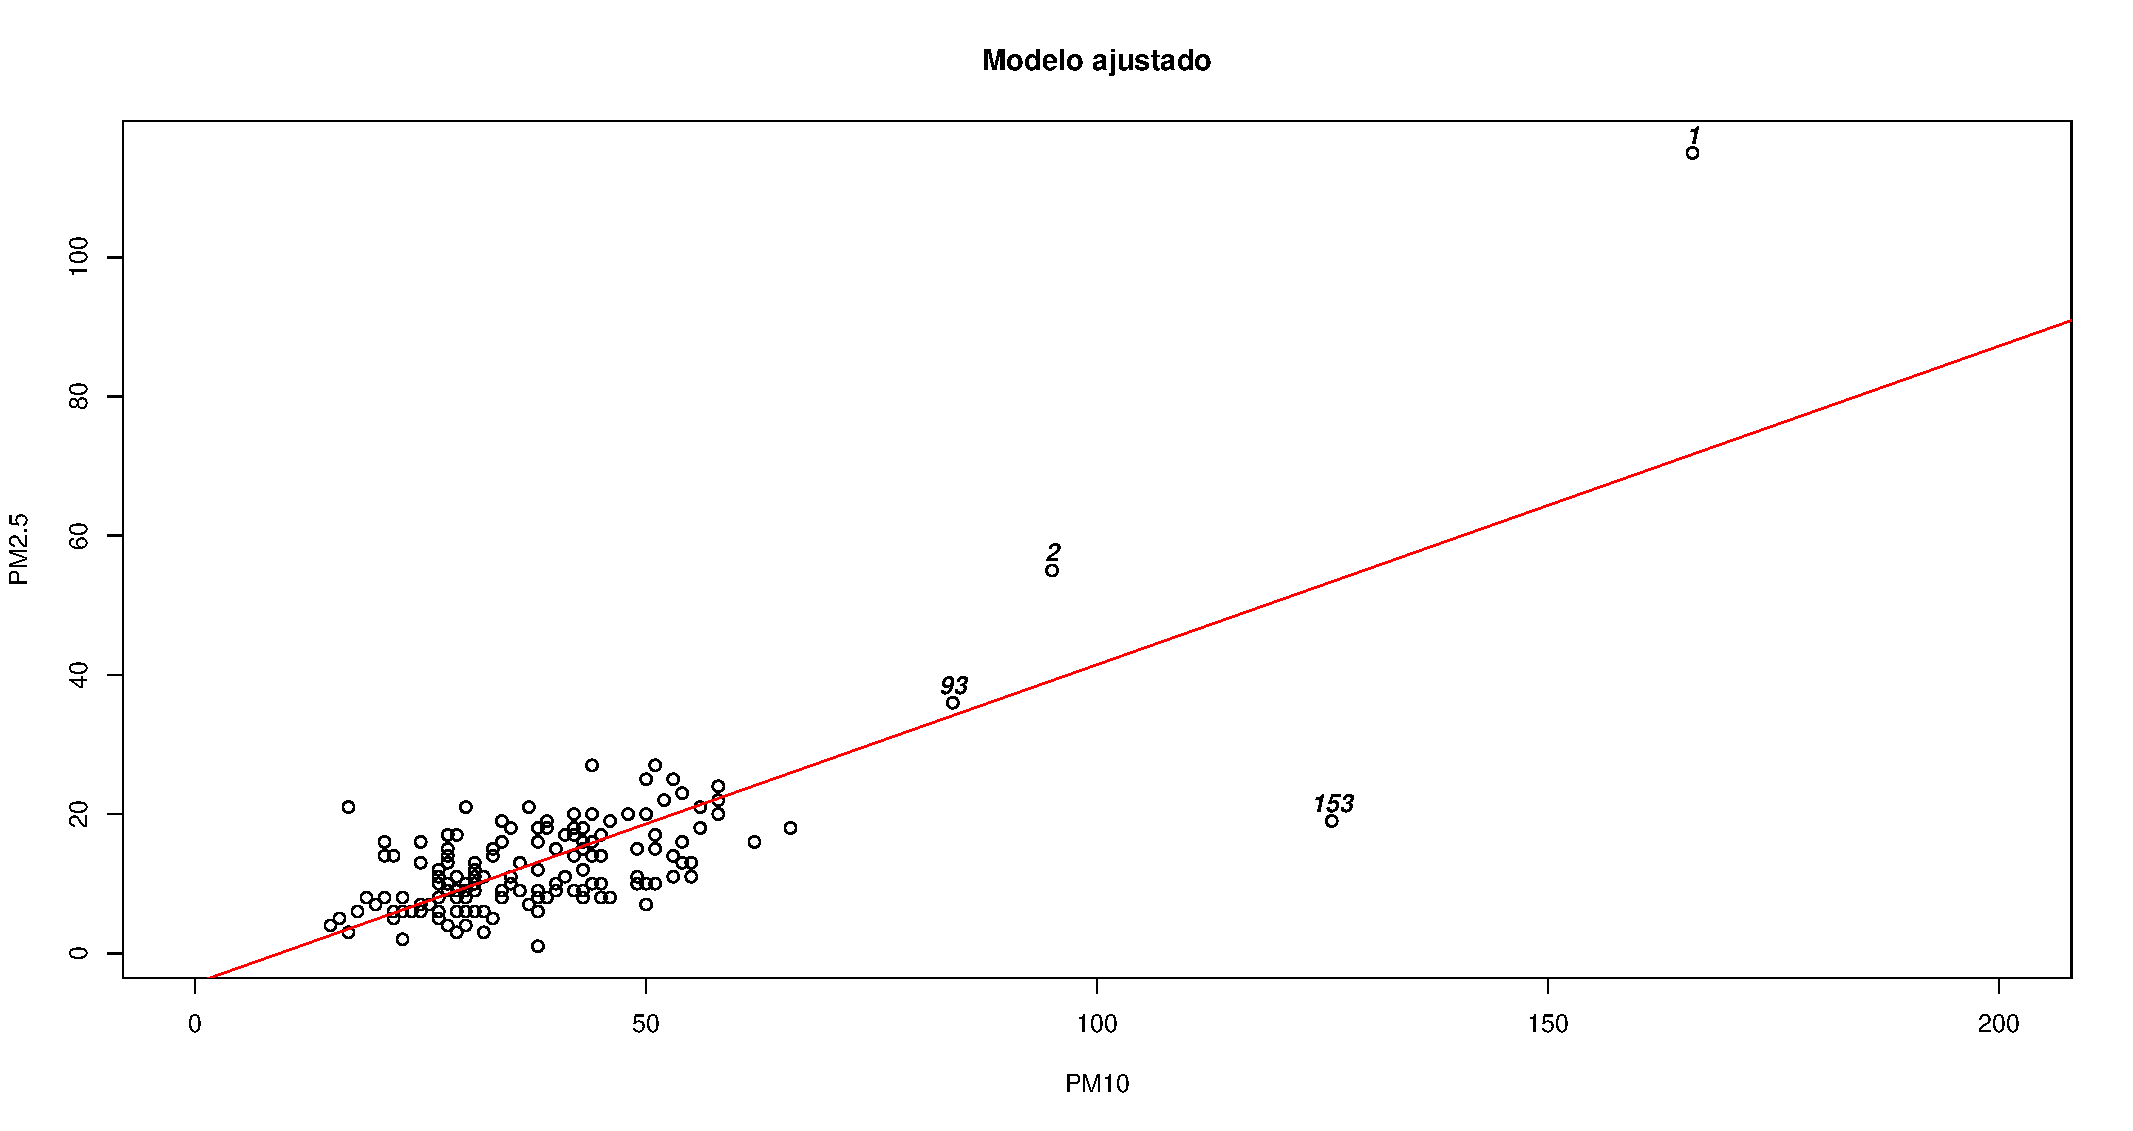
\includegraphics[scale=0.39]{imagenes/ma.pdf}
  \caption{Gráfico de dispersión con recta ajustada y valores candidatos a atipicos}\label{figura1}
\end{figure}
\end{itemize}
\end{frame}

\begin{frame}
\frametitle{Pruebas de diagnostico}
\begin{itemize}
\item[b)] \textbf{Gráfica de $\hat{d}$ vs $\hat{y}$:}
\begin{figure}[h]
  \centering
  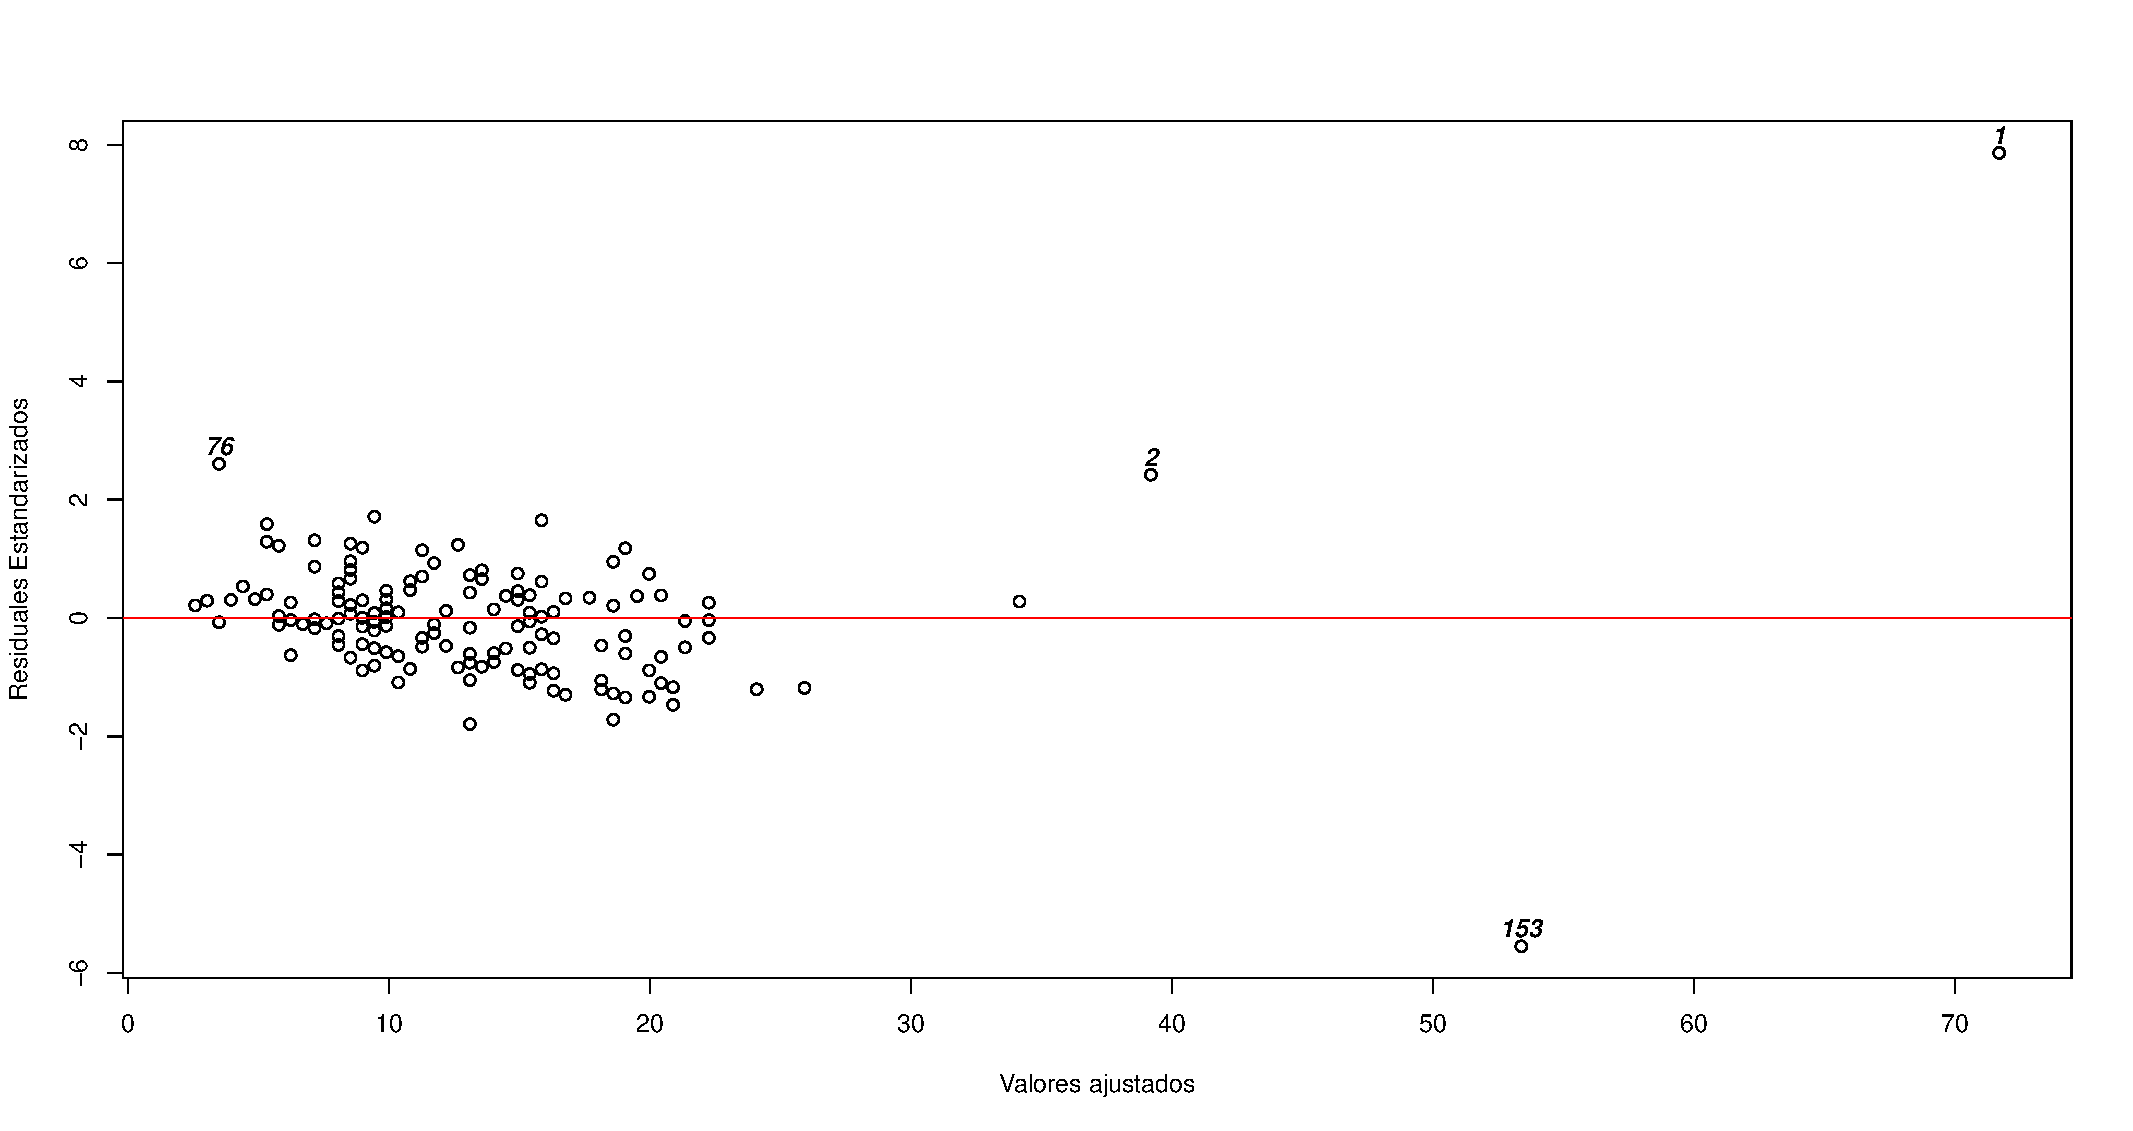
\includegraphics[scale=0.39]{imagenes/rv.pdf}
  \caption{Gráfico de residuales estandarizados vs los valores ajustados}\label{figura1}
\end{figure}
\end{itemize}
\end{frame}

\begin{frame}
\frametitle{Pruebas de diagnostico}
\begin{itemize}
\item[c)] \textbf{q-qplot de los residuales :}
\begin{figure}[h]
  \centering
  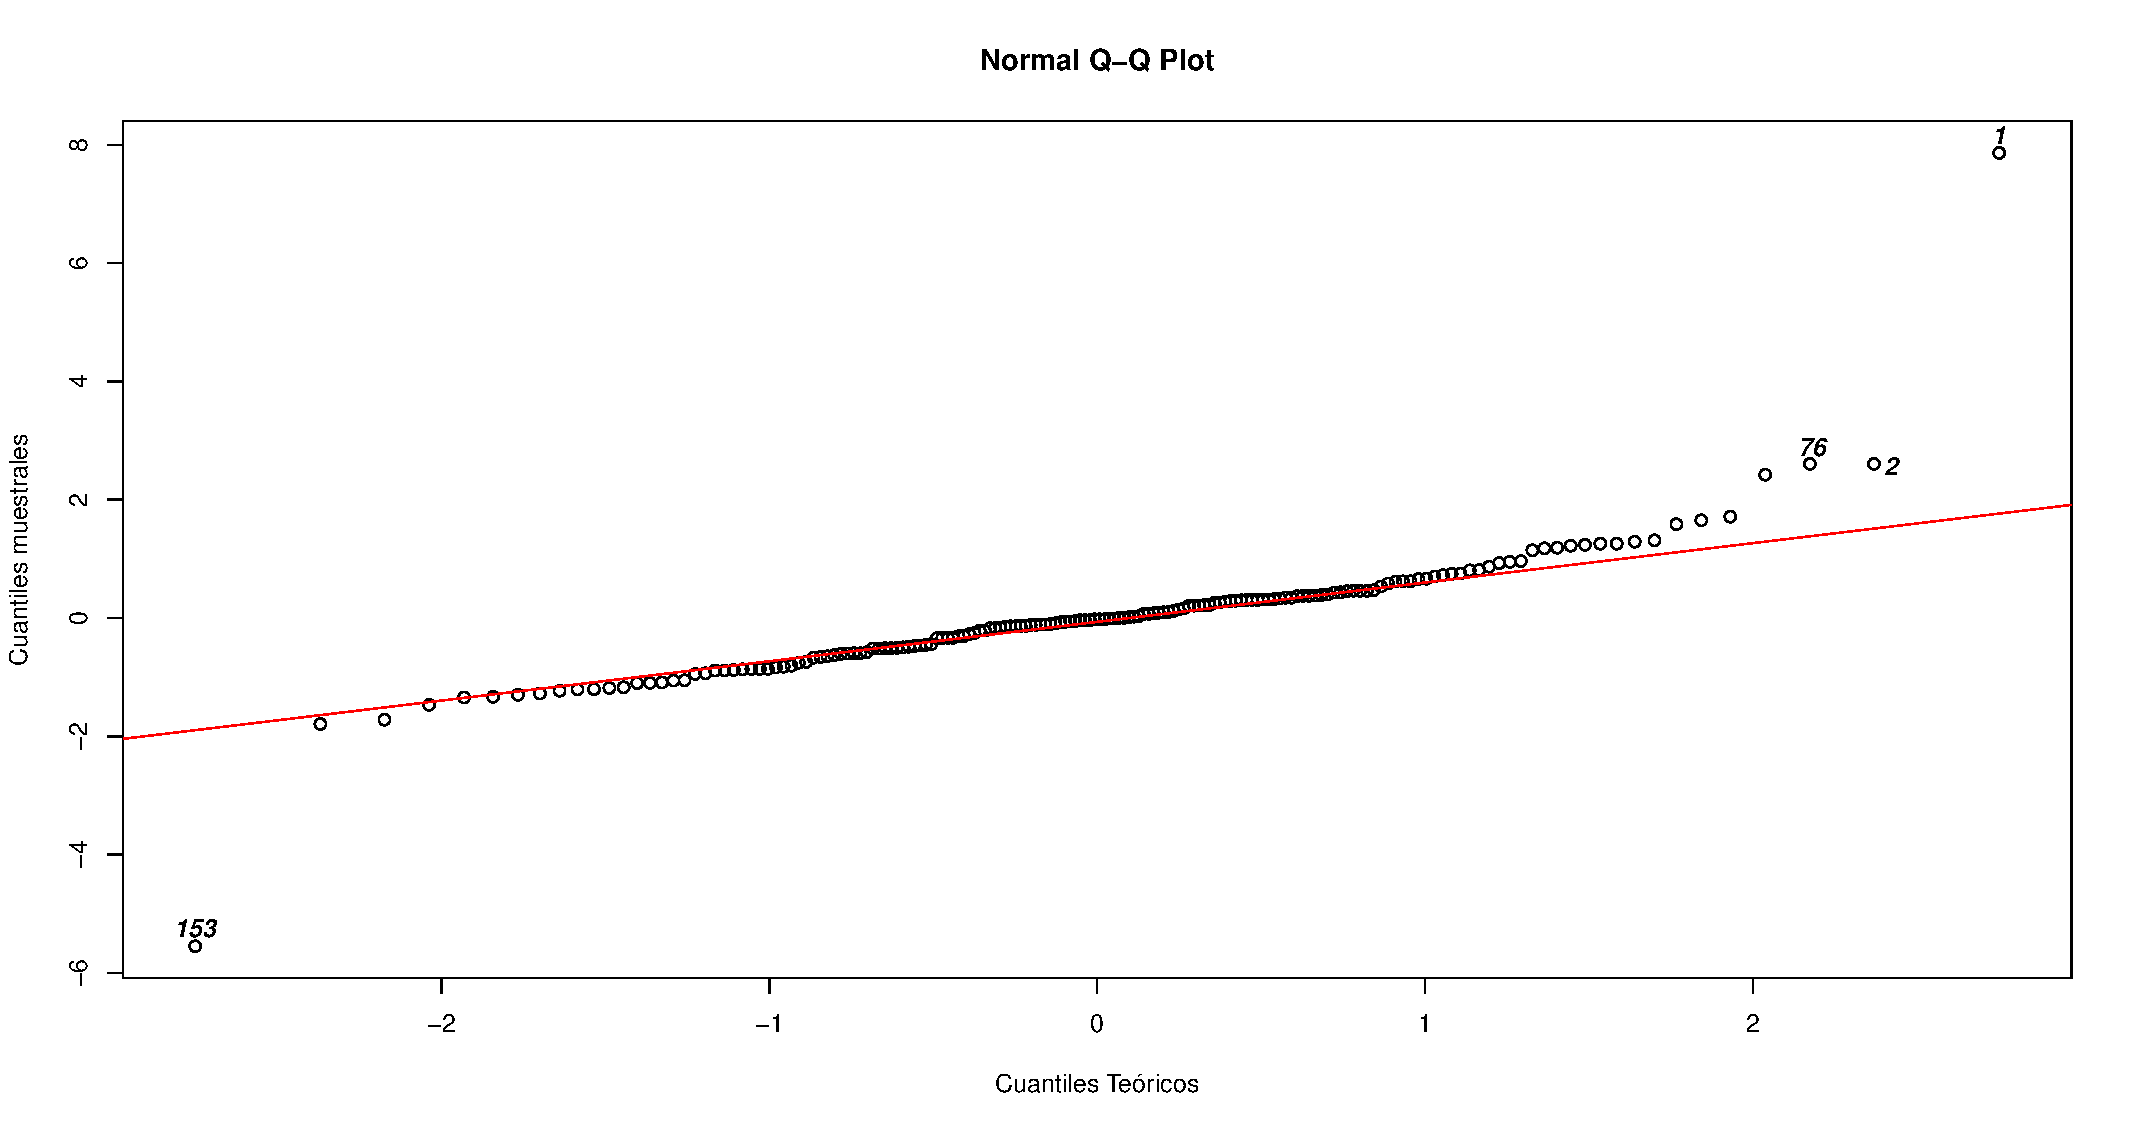
\includegraphics[scale=0.35]{imagenes/qq.pdf}
  \caption{q-qplot de los residuales}\label{figura1}
\end{figure}
\end{itemize}
\end{frame}

\begin{frame}
\frametitle{Pruebas de diagnostico}
\begin{itemize}
\item[d)] \textbf{Matriz HAT y residual Studentizado:} La matriz HAT definida como $H=x(x'x)^{-1}x^{T}$ y más específicamente el i-ésimo valor de su diagonal $h_{ii}=x'_{i}(X'X)^{-1}x_{i}$ y el residual Studentizado, definido como $\hat{r_{i}}=\frac{\hat{e_{i}}}{\sqrt{1-h_{ii}}\hat{\sigma}}$ sirven para ver si los puntos pueden ser influyentes o solo de balanceo, considerando los siguientes criterios:
\begin{itemize}
\item[-] Si $h_{ii}>\frac{2p}{n}=2\bar{h}=0.02381$ (como $\sum h_{ii}=p \rightarrow \bar{h}=\frac{p}{n}$) y el residual Studentizado es grande ($>3$), entonces la i-ésima observación puede considerarse influyente.
\item[-] Si solamente $h_{ii}>\frac{2p}{n}=0.02381$, entonces la i-ésima observación es solo de balanceo.
\end{itemize}
\end{itemize}
\end{frame}

\begin{frame}
\frametitle{Pruebas de diagnostico}
\begin{itemize}
\item[e)] \textbf{Distancia de Cook (D de Cook):} La distancia de Cook mide cómo cambia el vector de estimadores $\hat{\beta}$ cuando se elimina cada observación, por lo cuál es una medida útil para considerar como influyente una observación. La D de Cook se define como $D_{i}(M;C)=\frac{(\hat{\vec{\beta_{(i)}}}-\hat{\vec{\beta}})^T M(\hat{\vec{\beta_{(i)}}}-\hat{\vec{\beta}})}{C}$; i=1,...,n, donde $M=X^{T}X$ y $C=p\hat{\sigma^2}$. El criterio es:
\begin{itemize}
\item[-] Si $D_{i}\geq 1$, entonces la i-ésima observación puede considerarse como influyente.
\end{itemize}
\end{itemize}
\end{frame}

\begin{frame}
\frametitle{Pruebas de diagnostico}
\begin{itemize}
\item[f)] \textbf{DFFITS:} $DFFITS_{i}$ es la cantidad de desviaciones estándar que cambia el valor ajustado $\hat{y_{i}}$ si se elimina la observación i. Este criterio no define exactamente si el punto es influyente o de balanceo, solo sugiere que se debe examinar la observación. Se define como $DFFITS_{i}=\frac{\hat{y_{i}}-\hat{y_{(i)}}}{\sqrt{S^2_{(i)}}h_{ii}}$ El criterio es:
\begin{itemize}
\item[-] Si $|DFFITS_{i}|>2\sqrt{\frac{p}{n}}=0.2182$, sugiere que se debe investigar la influencia de la i-ésima observación.
\end{itemize}
\end{itemize}
\end{frame}

\begin{frame}
\frametitle{Pruebas de diagnostico}
\begin{itemize}
\item[g)] \textbf{DFBETAS:} Los $DFBETAS_{j,i}$ indica cuánto cambia el coeficiente de regresión $\hat{\beta_{j}}$ , en unidades de desviación estándar, si se omitiera la i-ésima observación. Esta se define como $DFBETAS_{ji}=\frac{\hat{\beta_{j}}-\hat{\beta_{j(i)}}}{\sqrt{S^{2}_{(i)}C_{jj}}}$ ; $C=(X^{T}X)^{-1}$. El criterio es:
\begin{itemize}
\item[-] Si $|DFBETAS_{ji}|>2/\sqrt{n}=0.1543$, entonces debe examinarse la i-ésima observación.
\end{itemize}
\end{itemize}
\end{frame}

\begin{frame}
\frametitle{Pruebas de diagnostico}
\begin{itemize}
\item[h)] \textbf{COVRATIO:} Esta medida sirve para expresar el papel de la i-ésima observación en la precisión de la estimación y se define como $\frac{|S^{2}_{(i)}(X^{T}_{i}X_{(i)})^{-1}|}{|S^{2}(X^{T}X)^{-1}|} $ ; i=1,2,...,n. El criterio es:
\begin{itemize}
\item[-] Si $COVRATIO_{i}>1$, entonces la i-ésima observación mejora la precisión de la estimación.
\item[-] Si $COVRATIO_{i}<1$, entonces la inclusión de la i-ésima observación disminuye la precisión de la estimación.
\item[-] Si $COVRATIO_{i}>1+3\frac{p}{n}=1.0357$  o si $COVRATIO_{i}<1-3\frac{p}{n}=0.9643$, entonces la i-ésima observación debería ser considerada influyente. 
\end{itemize}
\end{itemize}
\end{frame}

\begin{frame}
\frametitle{Resultados medidas de influencia}
\begin{center}
\resizebox{12.2cm}{!} {
\begin{tabular}{|cccccccc|}
\hline 
Observación & HAT & $\hat{r_{i}} $ &$D_{i}$ & $DFFITS_{i}$ & $DFBETAS_{(0),i}$ & $DFBETAS_{1,j}$ & $COVRATIO_{i}$ \\ 
\hline 
1 & 0.3384* & 9.8987499* & 15.8* & 7.07945* & -6.014452* & 7.02* & 0.602* \\ 
2 & 0.07179* & 2.4606893 & 0.227 & 0.684351* & -0.516887* & 0.655* & 1.015 \\  
76 & 0.01497 & 2.6539008 & 0.0516 & 0.327122* & 0.316146* & -0.254* & 0.945* \\  
79 & 0.01497 & 2.6539008 & 0.0516 & 0.327122* & 0.316146* & -0.254* & 0.945* \\ 
93 & 0.04881* & 0.2790688 & 0.00201 & 0.063217 & -0.044971 & 0.0592 & 1.063* \\ 
153 & 0.16301 & -6.1311115* & 3* & -2.705776* & 2.210180* & -2.66* & 0.802* \\ 
\hline 
\end{tabular} 
}
\end{center}
~\\Se puede observar que todas las observaciones de la tabla, se podrían considerar influyentes por uno u otro criterio.
\end{frame}

\begin{frame}
\frametitle{Modelo con intercepto 0}
~\\El modelo planteado para que pase por el origen es: 
$$PM_{2.5}=\beta_{1}PM_{10}$$
~\\El modelo ajustado asumiendo que el intercepto es igual a cero es: 
$$\hat{PM_{2.5}}=0.3638 PM_{10}$$
\end{frame}

\begin{frame}
\frametitle{Bondad del modelo}
~\\Para este modelo ajustado, tenemos los siguientes resultados que nos ayudaran a juzgar que tan bueno es:
\begin{center}
\begin{tabular}{|c|c|c|c|c|}
\hline 
 & Estimación & Desviación Estandár & Estadistico T & P valor \\ 
\hline 
$\beta_{1}$ & 0.3638 & 0.0129 & 28.2 & $<2e-16$ \\ 
\hline 
\end{tabular} 
\end{center}
\begin{center}
\begin{tabular}{|c|c|c|c|c|}
\hline 
$R^2$ & $R^2_{Ajustado}$ & $\hat{\sigma}$ & Estadistico F & Valor p \\ 
\hline 
0.8265 & 0.8254 & 6.978 & 795.4 & $<2.2e-16$ \\ 
\hline 
\end{tabular} 
\end{center}
\end{frame}

\begin{frame}
\frametitle{Comparación de modelos}
\begin{figure}[h]
  \centering
  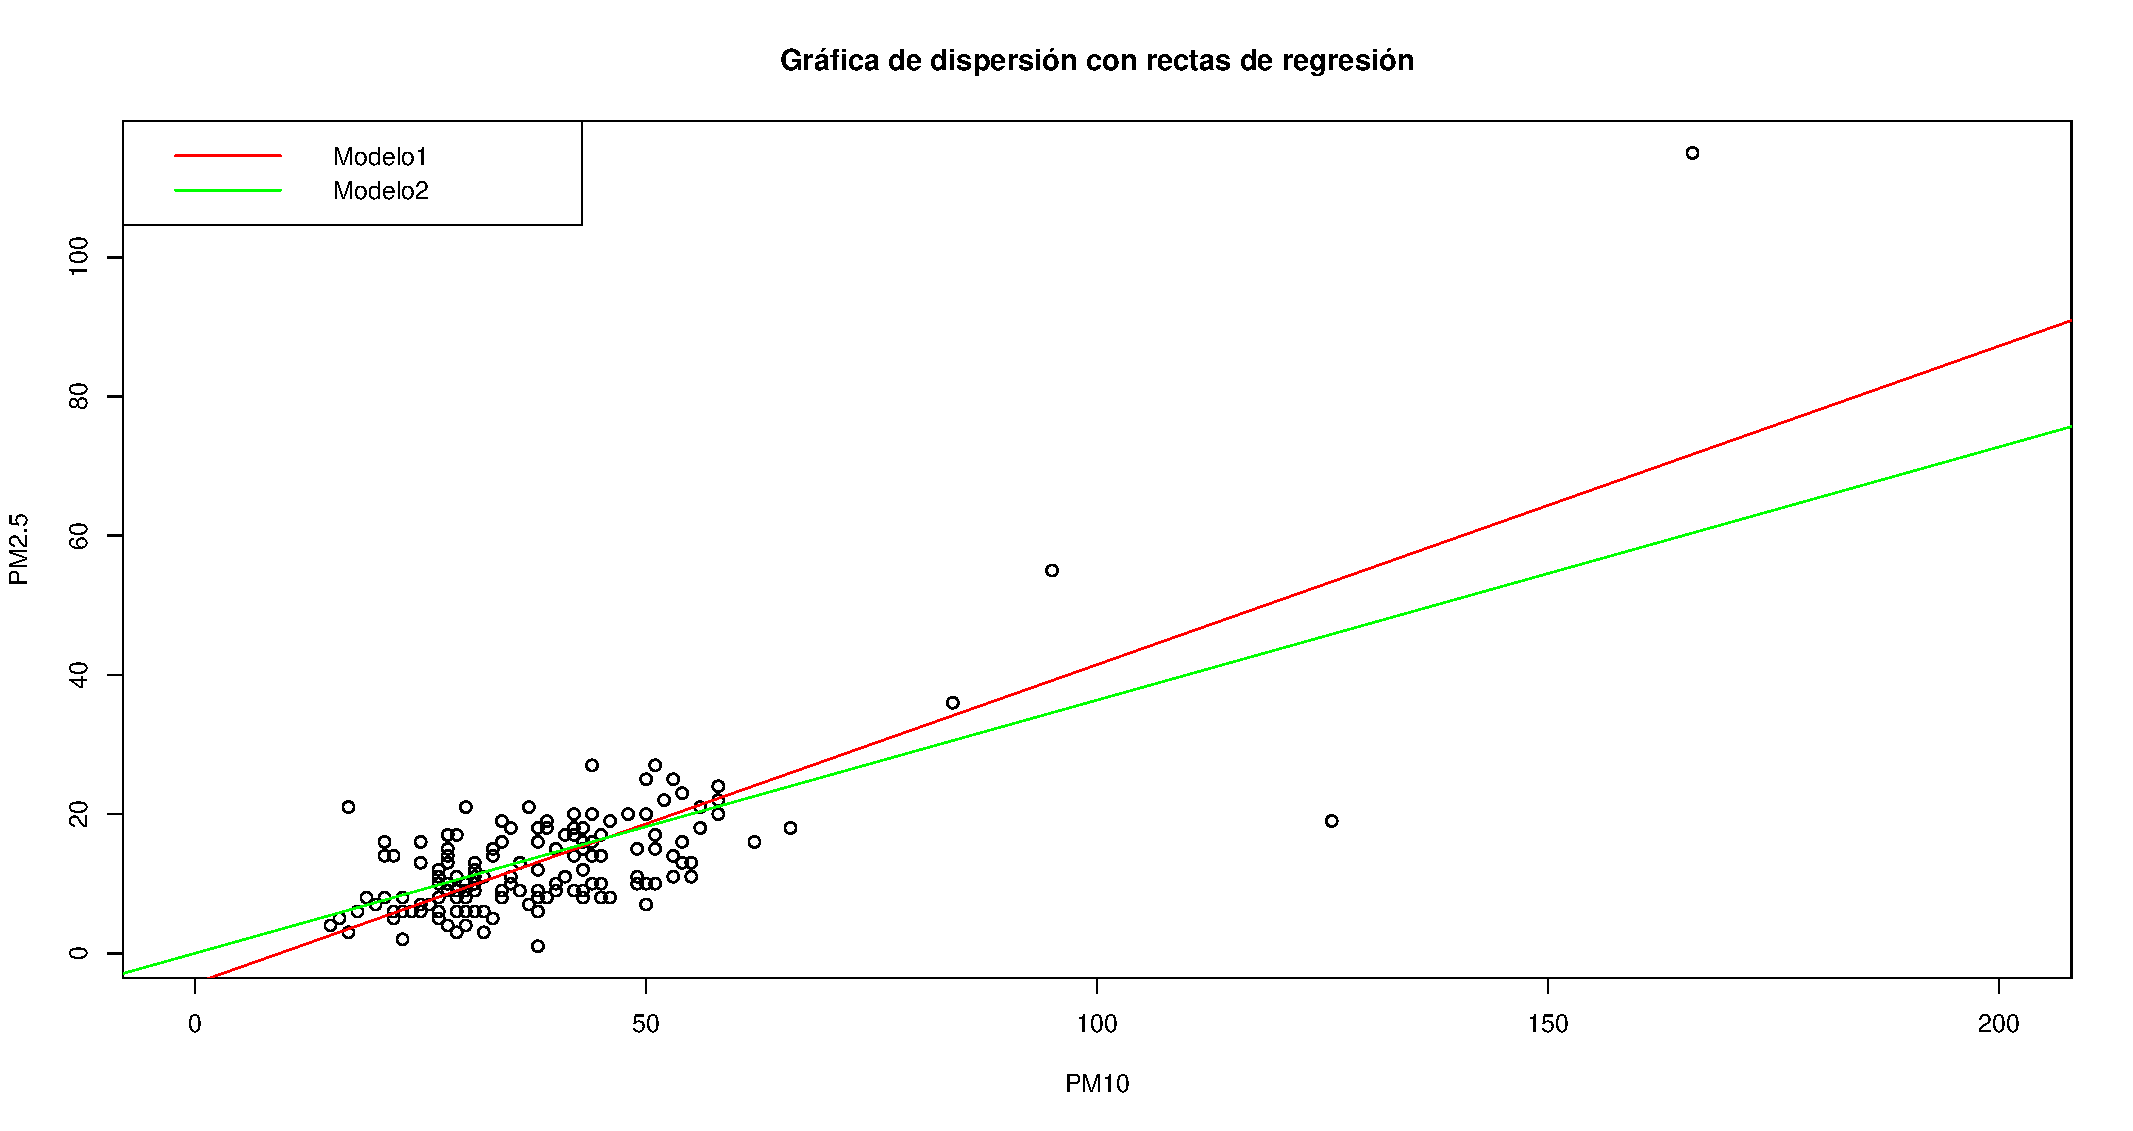
\includegraphics[scale=0.35]{imagenes/comp.pdf}
  \caption{Gráfica comparativa de rectas de regresión}\label{figura1}
\end{figure}
\end{frame}

\begin{frame}
\frametitle{Comparación de modelos}
~\\Para comparar los modelos tenemos la siguiente tabla comparativa:
\resizebox{12.2cm}{!} {
\begin{tabular}{|c|c|c|c|c|c|c|c|}
 \hline 
 Modelos & $R^{2}_{Ajustado}$ & $\hat{\sigma}$ & Estadistico F & Valor P & AIC & BIC & $SD(\beta_{1})$ \\ 
 \hline 
 Modelo 1 & 0.5729 & 6.7707 & 225 & $<2.2e-16$ & 1123.39 & 1132.762 & 0.45776  \\ 
 \hline 
 Modelo 2 & 0.8254 & 6.978 & 795.4 & $<2.2e-16$ & 1132.546 & 1138.794 & 0.3638\\ 
 \hline 
 \end{tabular}
 }  
\end{frame}

\begin{frame}
\frametitle{Comparación modelos}
~\\Seleccionamos como mejor modelo, al segundo, en el cuál se asumió que el intercepto es igual a 0. Se hizo esa elección ya que viendo el $R^2$ y el $R^2_{Ajustado}$, hubo un aumentó bastante grande en ambos (cerca del 0.25) lo cuál es muy bueno, ya que nos dice que la variabilidad del $PM_{2.5}$ explicada por el $PM_{10}$ aumentó en un $25\%$ asumiendo que el intercepto es 0. Además, si nos fijamos en la desviación estándar de la estimación, vemos que se hace más pequeña, lo cuál quiere decir que la precisión de la estimación aumentó y, por último, la prueba de significancia también se rechazo, es decir, $\beta\neq 0$, por lo tanto, el modelo es significativo. Hubo un aumento en la desviación estándar de 0.2, lo cuál no nos pareció una razón de peso para no elegirlo.
\end{frame}

\begin{frame}
\frametitle{Pruebas de diagnostico modelo 2}
~\\Los resultados de las medidas de influencia y las pruebas de diagnostico para este modelo se resumen en la siguiente tabla:

\begin{center}
\resizebox{12.2cm}{!} {
\begin{tabular}{|ccccccc|}
\hline 
Observación & HAT & $\hat{r_{i}} $ &$D_{i}$ & $DFFITS_{i}$ & $DFBETAS_{1,j}$ & $COVRATIO_{i}$ \\ 
\hline 
1 & 0.094157* & 10.625441* & 7.03* & 3.43* &  3.43* & 0.661* \\ 
2 & 0.03084* & 3.048048* & 0.282 & 0.544* & 0.544* & 0.983 \\  
76 & 0.000987 & 2.146917  & 0.00446 & 0.0675 &  0.0675 & 0.980* \\  
79 & 0.000987 & 2.146917 & 0.00446 & 0.0675  & 0.0675 & 0.980* \\ 
93 & 0.024110* & 0.788304 & 0.0154 & 0.124  & 0.124 & 1.027* \\ 
153 & 0.054247* & -4.141674*  & 0.897 & -0.992*  & -0.992* & 0.964* \\ 
\hline 
\end{tabular} 
}
\end{center}
\end{frame}

\begin{frame}
\frametitle{Validación de supuestos, modelo 2}
\begin{itemize}
\item[a)] Correcta especificación (Linealidad): Para evaluar la correcta especificación del modelo, simplemente nos basamos en las siguientes dos gráficas. 
\begin{figure}[h]
  \centering
  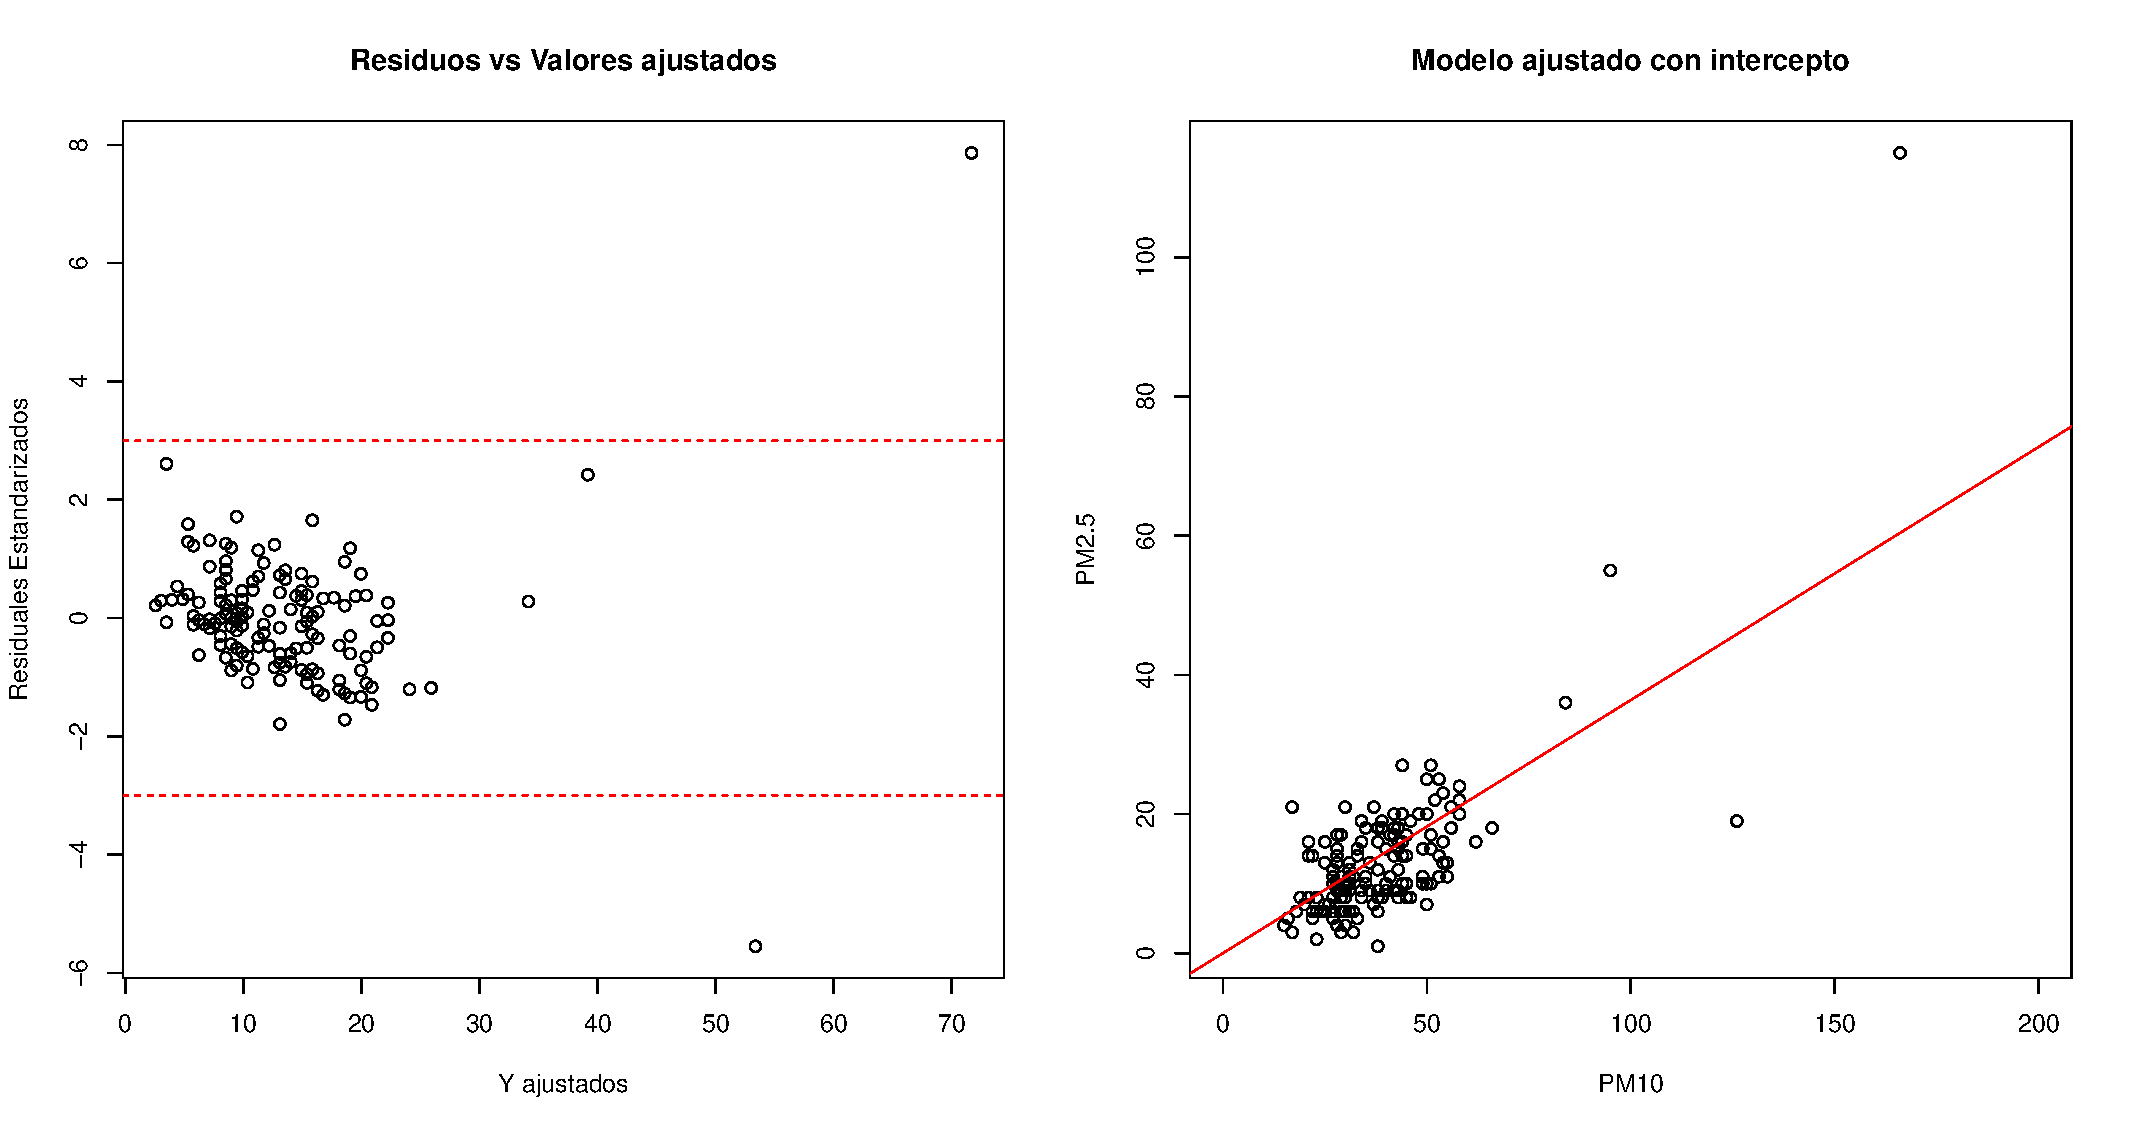
\includegraphics[scale=0.31]{imagenes/coresp.pdf}
  \caption{Gráficos para detectar incorrecta especificación }\label{figura1}
\end{figure}
\end{itemize}
\end{frame}

\begin{frame}
\frametitle{Validación de supuestos, modelo 2}
\begin{itemize}
\item[b)] Normalidad de los errores: Para verificar este supuesto, se realizaron nuevamente dos gráficas, la primera, un histograma de los residuales para ver una posible forma de distribución de estos, y la segunda, el Q-Qplot, que muestra que tanto se asemeja la distribución de los residuales a la distribución normal. En ambas gráficas se evidencia que la distribución de los residuales no es normal, se puede ver en ambas que la cola derecha de la distribución de los residuales es mucho más pesada que en la distribución normal. Además aplicamos la prueba Shapiro-Wilk para confirmar nuestra creencia, esta prueba nos arrojo un estadistico de $W = 0.77708$ y un p valor= 1.032e-14, por tanto se rechaza $H_{0}$ y se concluye que la distribución de los residuales no es normal.
\end{itemize}
\end{frame}

\begin{frame}
\frametitle{Validación de supuestos, modelo 2}
\begin{figure}[h]
  \centering
  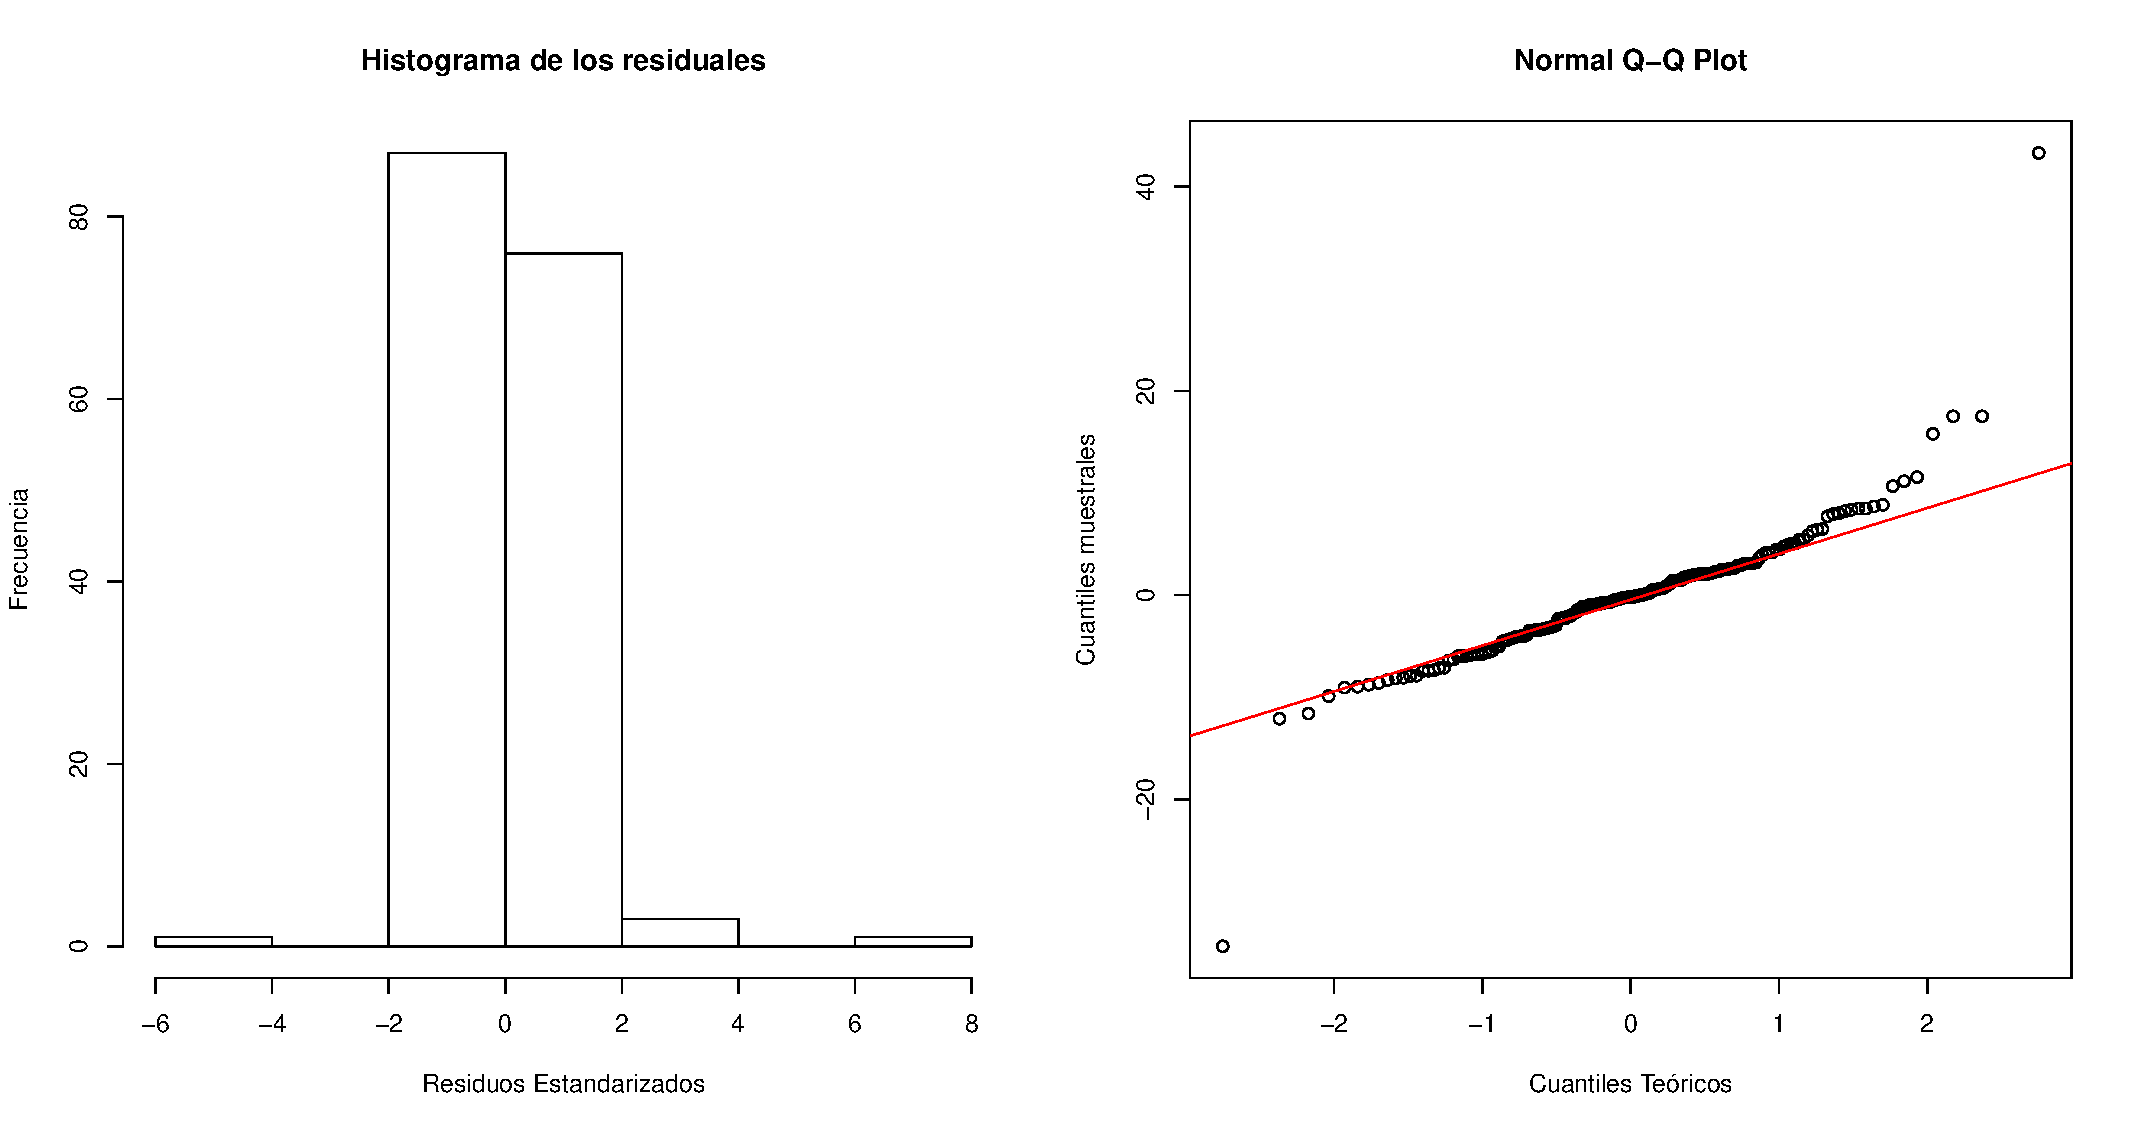
\includegraphics[scale=0.37]{imagenes/norm.pdf}
  \caption{Gráficos para evaluar la normalidad en los errores}\label{figura1}
\end{figure}
\end{frame}

\begin{frame}
\frametitle{Validación de supuestos, modelo 2}
\begin{itemize}
\item[c)] Homocedasticidad: Para probar la homocedasticidad, se analiza la misma gráfica realizada en el literal a (los residuales vs los $\hat{y}$ donde se ve que las varianzas son muy parecidas, por lo cual se sospecha que se cumple este supuesto, sin embargo se realizó también la prueba Goldfeld-Quandt, se eligió esta, ya que todas las otras pruebas conocidas (Levene, Barlett, Cochran, Breusch-Pagan, etc) algunas requieren repeticiones en X y otros supuestos, y otras requieren o necesitan el intercepto (es el caso de la prueba de Breusch-Pagan) y este modelo no tiene intercepto. La prueba Goldfeld-Quandt nos arrojo un estadístico de prueba $GQ = 0.44682$ y un p valor de 0.9998. Por lo cuál no se rechaza la hipotesis nula,y concluimos que los residuos del modelo no dan evidencia para decir que tienen heterogeneidad de varianza.
\end{itemize}
\end{frame}


\end{document}